
%
% foundations - mapping
%

\section{Web Mapping}

Maps have become an almost instinctive way of seeing our world. They probably first appeared over 18,000 years ago and already in the 1500s, they were produced in large numbers for navigational and military purposes. Maps are powerful tools that help organize boundaries and administrative activities. They allow telling stories, visualizing data and understanding geographic contexts
~\cite{Zzolo11mappingdrupal}.

Recently, Google Maps\footnote{\url{http://maps.google.com}} has made digital maps available to a large number of internet users. Digital natives are used to navigate using interactive maps on their smart phones and look up places on online maps on their computers.

Web mapping describes the whole process of designing, implementing, generating and delivering maps on the internet. It applies theoretical foundations from web cartography to the technical possibilities and boundaries of constantly evolving web technologies. The continuous development of related technologies has created a wide variety of \textit{types of web maps}: from analytic, animated, collaborative and dynamically created web maps to online atlases, realtime and static web maps~\cite{wiki:web-mapping}.

\subsection{Map Projections}

The planet earth is a roughly spherical geoid. In order to represent it on flat computer screens, the surface of the earth needs to be translated to a plane. This is realized by applying the method of a map projection. Choosing a map projection influences how shapes, areas, directions and distances will be preserved or distorted. As no projection can optimize all those factors at once, choosing the right projection depends on the purpose of the map.

The \textit{spherical mercator projection} is the most commonly used web mapping projection. It preserves shapes and direction, but does this at the cost of enlarging areas towards the poles. This distortion can be visualized by Tissot's indicatrix. Figure \ref{fig:mercator} shows how circles of the same relative size get extrapolated off the equator by using the mercator projection~\cite{Zzolo11mappingdrupal, wiki:web-mapping}. 

\begin{figure}[h]
  \begin{center}
    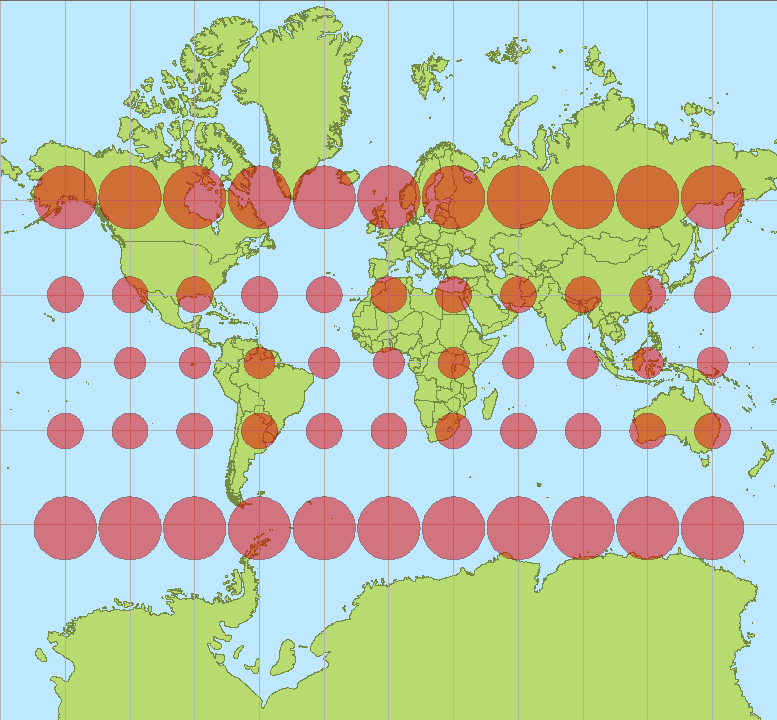
\includegraphics[width=0.5\textwidth]{figures/tissot_mercator.png}
    \caption{Tissot's indicatrix visualizes enlarged areas towards the poles when using the mercator projection~\cite{wiki:mercator}.}
    \label{fig:mercator}
  \end{center}
\end{figure}


\subsection{Coordinates}

In mapping, a coordinate system is used when representing locations in a numeric way. The primary way to store coordinates of locations is a pair of \textit{latitude} and \textit{longitude} values. 

\begin{itemize}

\item \textbf{Latitude} classifies the angular distance towards north and south from the equator which is at $0^\circ$. Positive latitude values represent the northern hemisphere up the the pole at $90^\circ$. Negative values are located below equator where the south pole marks the lower limit at $-90^\circ$.

\item \textbf{Longitude} denotes the angular distance towards west and east. It's zero-mark is a latitude of $0^\circ$  which runs north-south through the Royal Observatory at Greenwich in the UK. In contrast to latitude values, the longitude encloses a whole circle around the earth. Negative values down to $180^\circ$ are located west and positive values up to $180^\circ$ are positioned east of Greenwhich.

\end{itemize}

In classic mapping applications, latitude and longitude values are measured in degrees, minutes and seconds of the sphere. New York City is located at $40^\circ$ $43'$ $0''$ North, $74^\circ$ $0'$ $0''$ West. For computational purposes, web mapping is largely based on a decimal degree representation of such values. The equivalent decimal degree value for New York in that case is the pair of $40.716667, -74$.

A common pitfall in web mapping is mixing up the order of latitude and longitude values. Having latitude before longitude is the standard, which means to state the vertical position before the horizontal. This contradicts with classic Cartesian x,y coordinate systems and often leads to confusion. Some mapping APIs expect latitude first, while others are designed to begging with longitude values~\cite{Zzolo11mappingdrupal}. 


\subsection{The Web Mapping Stack}

The primary purpose of web mapping applications is to deliver spatial data in the form of a map to the user. Modern, interactive web mapping applications are based on a concept named \textit{slippy maps}. Slippy maps are displayed in a rectangular viewport within the browser handled by a javascript mapping library. The map is visualized dynamically by rendering layers of raster and vector data on top of each other. In addition, slippy maps provide means of interaction to the user such as panning and zooming to update and explore the map. Figure \ref{fig:web-mapping-stack} illustrates the prototype of such a modern web mapping application. Its components will be discussed in the following section.

\begin{figure}[h]
  \begin{center}
    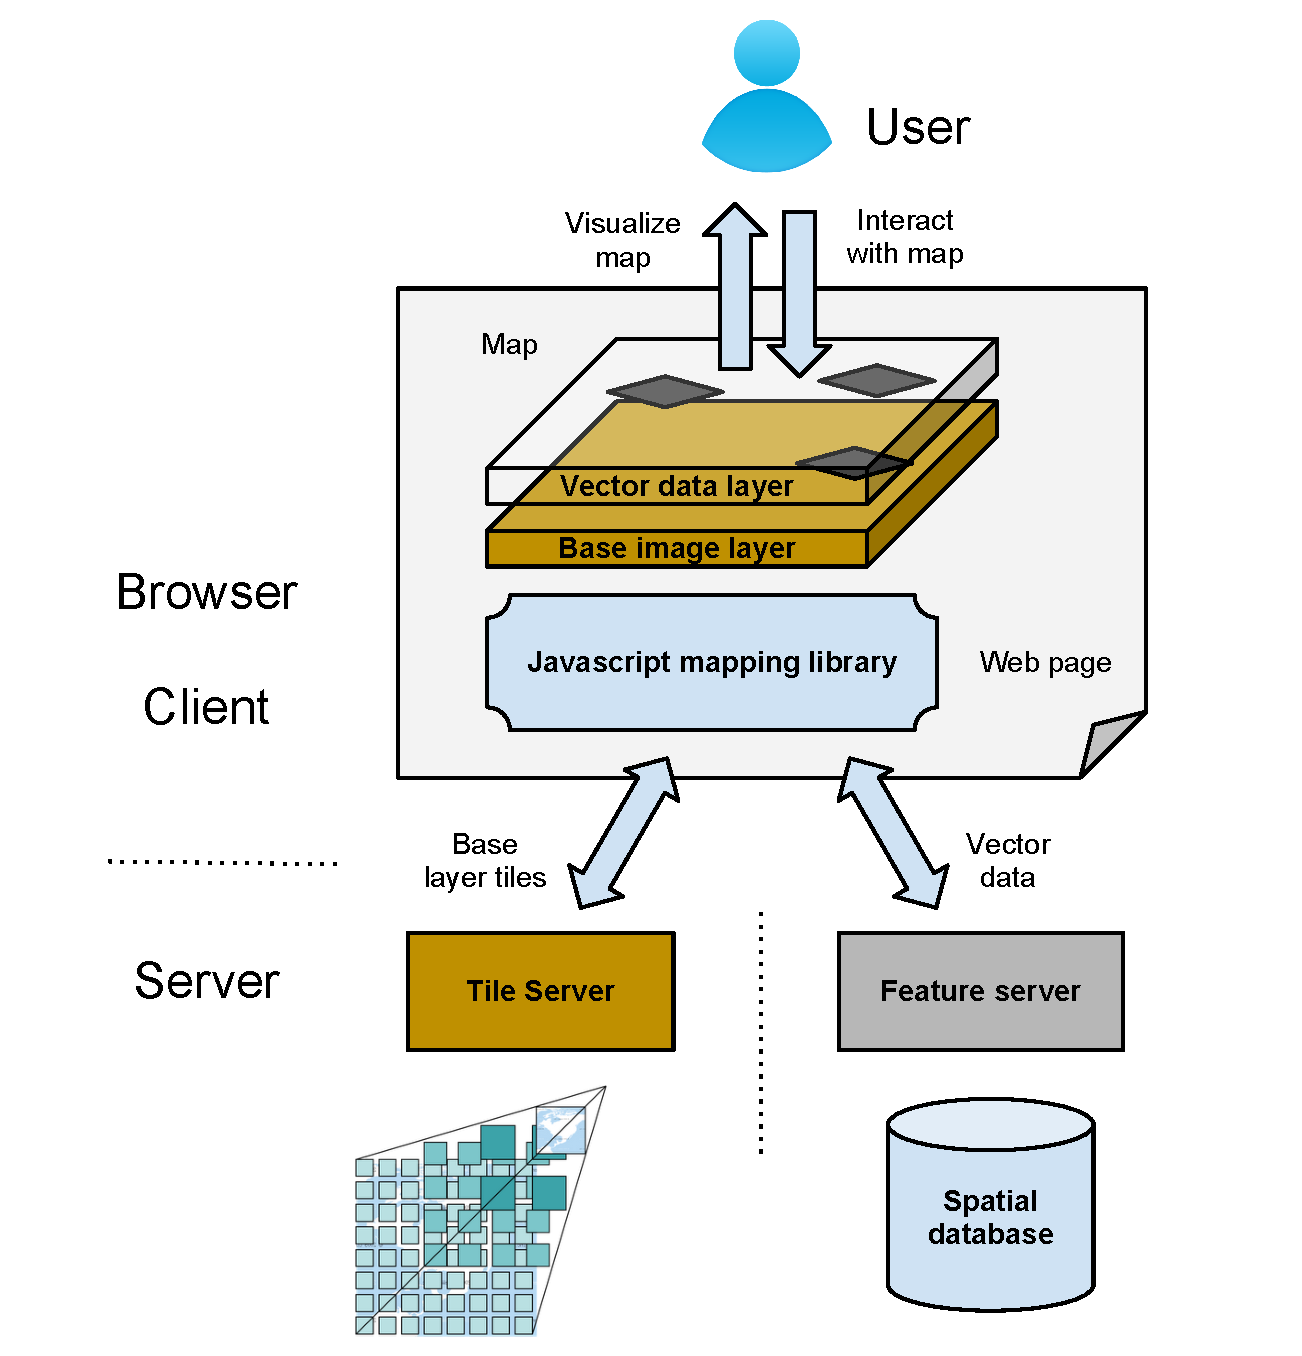
\includegraphics[width=1\textwidth]{figures/web_mapping_stack.pdf}
    \caption{Illustration of a modern web mapping application. Includes a tile graphic from~\cite{web:cubeservtiles}.}
    \label{fig:web-mapping-stack}
  \end{center}
\end{figure}















